\documentclass[10pt]{article}
\usepackage[margin=0.8in]{geometry}
\usepackage{amsmath,amssymb,booktabs,graphicx}
\usepackage[font=small]{caption}
\setlength{\parskip}{3pt}\setlength{\parindent}{0pt}
\graphicspath{{figures/}{../results/}}
\title{Finite-Time Swarm Tracking: Numerical Results}
\author{}\date{}
\begin{document}
\maketitle\vspace{-2em}
\IfFileExists{../results/experiment_4/report_metrics.tex}{\newcommand{\MapACount}{0}
\newcommand{\MapBCount}{14}
\newcommand{\MapCCount}{2}
\newcommand{\MapDCount}{0}
\newcommand{\MapFailureCount}{0}
\newcommand{\MapTotalCases}{16}
\newcommand{\MapGridSize}{4}
\newcommand{\MapMinSeparation}{0.909082}
\newcommand{\MapMinPeak}{9.78177}
\newcommand{\MapMaxPeak}{37.378}
\newcommand{\MapDisconnectedCount}{0}
\newcommand{\MapSeparationCount}{2}
}{\newcommand{\MapACount}{0}
\newcommand{\MapBCount}{14}
\newcommand{\MapCCount}{2}
\newcommand{\MapDCount}{0}
\newcommand{\MapFailureCount}{0}
\newcommand{\MapTotalCases}{16}
\newcommand{\MapGridSize}{4}
\newcommand{\MapMinSeparation}{0.909082}
\newcommand{\MapMinPeak}{9.78177}
\newcommand{\MapMaxPeak}{37.378}
\newcommand{\MapDisconnectedCount}{0}
\newcommand{\MapSeparationCount}{2}
}

All quantities are normalized. This report retains the arbitrary
formation demonstration (Exp.~1), the finite-time convergence and coupling gain
evaluation (Exp.~2), the star-formation safety and connectivity transient
comparison across three representative cases (Exp.~3), and the Experiment 4
coupling--speed parameter sweep.

\section{Model and parameters}
The physical agents use
\[
\dot x_i=u_i=\dot q_i-\delta_i-\operatorname{sig}^{\beta}(\delta_i)
-\sum_jw_{ij}M(\delta_i-\delta_j),\qquad \delta_i=x_i-q_i,
\]
where $\operatorname{sig}^{\beta}(z)=\operatorname{sign}(z)|z|^{\beta}$,
$M=mI_2$, $\beta=0.5$, and
$w_{ij}=a_{ij}/(\|x_i-x_j\|+0.2)$ with $a_{ij}=1$ if $\|x_i-x_j\| < R_c$ ($i \neq j$) and $0$ otherwise. No centroid feedback, state reset, or
controller smoothing is used. The ten centered star stations are
\begin{align*}
q_i(t)&=r(t)+a(t)p_i^0,&a(t)&=a_\infty+(1-a_\infty)e^{-0.9t},\quad a_\infty=1.65-0.25\kappa,\\
r(t)&=[0.9t,1.1\sin(0.35t)]^T,&
\dot r(t)&=[0.9,0.385\cos(0.35t)]^T,
\end{align*}
with $p_i^0=b_i[\cos\phi_i,\sin\phi_i]^T$,
$\phi_i=\pi/2+\pi i/5$, and $b_i=2.8$ for even $i$ and $1.22$ for odd
$i$, $i=0,\ldots,9$, centered so $\sum_i p_i^0 = 0$. The tightest station pair has distance $DQ_0 = 1.4342$, and the template diameter is $\ell_{H,0} = 5.3259$. Station velocities are analytic. The full horizon is $t_f = 12.0$, and the safety and connectivity transients are analyzed over $t \in [0, 2.5]$. The safety threshold is $d_{\rm safe}=0.95$, and the communication radius is $R_c=6.60$.

The initial tracking perturbation $\delta_i(0)$ is zero-mean ($\sum_i \delta_i(0)=0$), generated from Gaussian noise with $\sigma=0.03$, with the closest template pair $(5,7)$ nudged inward by $0.12$ and the farthest pair $(0,4)$ nudged outward by $0.22$. This gives initial error norm $\|\delta_0\| = 0.3712$, effective distortion $\rho_{\rm eff,0} = 0.4185$, and universal deadline $\overline T_{\rm univ} = 2\ln(1+\sqrt{\|\delta_0\|}) = 0.9515$.

The time-varying geometric margin is
\[
s(t) = \min\{a(t)DQ_0 - d_{\rm safe},\; R_c - a(t)\ell_{H,0}\}.
\]
For coupling gain $m$, the effective rate is $\gamma = 1 + m w_{\rm lower}\lambda_2(L_H)$ with $w_{\rm lower} = 1/(R_c+\epsilon_w) = 1/6.8$ and $\lambda_2(L_H) = 10$. The distortion bound is
\[
\rho_H(t) = \min\{\sqrt{2}\overline R(t, \gamma),\; \rho_{\rm eff,0}e^{-\gamma t}\},\qquad
\overline R(t, \gamma) = \max\left\{0, \left(\frac{(1+\gamma\sqrt{\|\delta_0\|})e^{-\frac{1}{2}\gamma t}-1}{\gamma}\right)^2\right\}.
\]
The required rate $\gamma_{\rm req}$ is evaluated over $\tau \in (0, \overline T_{\rm univ}]$ by maximizing $\frac{\ln(\rho_{\rm eff,0}/s(\tau))}{\tau}$.

\section{Formation demonstration}
The original ring--wedge--star--arrow example uses smooth quintic blends and
analytic station derivatives. It demonstrates tracking of reconfiguring
formations; it makes no general collision-avoidance claim.
\begin{figure}[ht]\centering
\IfFileExists{../results/experiment_1/formation_snapshots.pdf}{\includegraphics[width=.78\linewidth]{experiment_1/formation_snapshots.pdf}}{\includegraphics[width=.78\linewidth]{formation_snapshots.pdf}}
\caption{Moving reference and reconfiguring formations.}
\end{figure}

\section{Finite-time tracking and coupling gain evaluation}
Experiment~2 evaluates the safe-certified star formation maneuver ($\kappa=3.0$, scale rate $0.90$) across coupling gains $m \in \{0, 0.5, 2, 2.5, 5, 10\}$. Figure~\ref{fig:exp2_errors} shows the station tracking error $\|\delta(t)\|_2$, the formation disagreement $\|\eta(t)\|_2$, and the physical control command $\|u(t)\|_2$. In panels (a) and (b), the curves are cut at $10^{-4}$, capturing the clean finite-time transient down to settling without plotting the post-convergence numerical discretization noise.

As coupling gain $m$ increases, formation disagreement decays substantially faster, accelerating overall settling time to the $10^{-6}$ error threshold from $0.7683$~s at $m=0$ down to $0.1883$~s at $m=10$ (Table~\ref{tab:star_gain}). All runs settle well within the theoretical universal deadline $\overline T = 0.9515$~s.

\begin{figure}[ht]\centering
\IfFileExists{../results/experiment_2/error_disagreement_control.pdf}{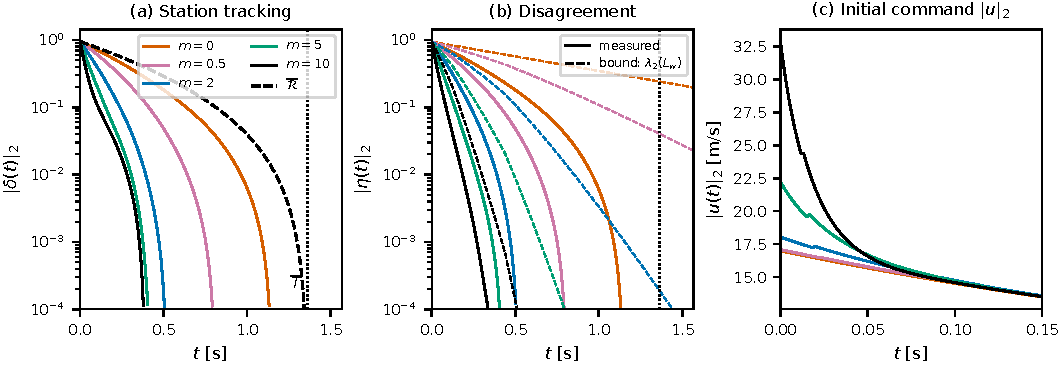
\includegraphics[width=.98\linewidth]{experiment_2/error_disagreement_control.pdf}}{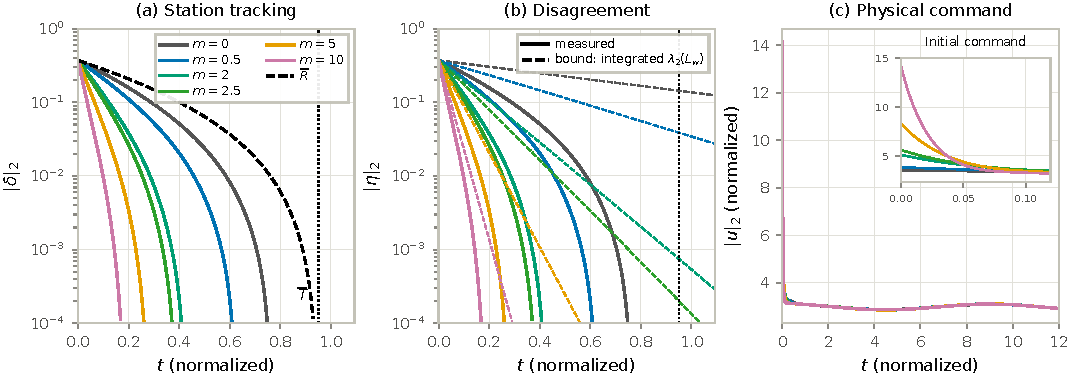
\includegraphics[width=.98\linewidth]{error_disagreement_control.pdf}}
\caption{Experiment 2 finite-time tracking and disagreement across coupling gains $m$ ($\kappa=3.0$). (a) Station tracking $\|\delta\|_2$ against universal bound $\overline R$ and deadline $\overline T$, cut at $10^{-4}$. (b) Disagreement $\|\eta\|_2$ against exponential rate bound, cut at $10^{-4}$. (c) Physical control command $\|u\|_2$ with initial transient inset.}
\label{fig:exp2_errors}
\end{figure}

\begin{table}[ht]\centering\footnotesize
\caption{Experiment 2: Settling times and control metrics across coupling gains $m$ under safe-certified star formation ($\kappa=3.0$).}
\IfFileExists{../results/star_gain_table.tex}{\begin{tabular}{rrrrr}\toprule
$m$ & $t_{10^{-6}}$ & $\overline T$ & $\max\|u\|_2$ & $J_u$\\\midrule
0 & 0.768333 & 0.951538 & 3.50984 & 0.32748 \\
0.5 & 0.628333 & 0.831398 & 3.82752 & 0.438974 \\
2 & 0.43 & 0.621194 & 5.10868 & 0.772248 \\
2.5 & 0.39 & 0.576439 & 5.60358 & 0.883193 \\
5 & 0.28 & 0.43254 & 8.30945 & 1.43756 \\
10 & 0.188333 & 0.300258 & 14.1435 & 2.54577 \\
\bottomrule\end{tabular}
}{\begin{tabular}{rrrrr}\toprule
$m$ & $t_{10^{-6}}$ & $\overline T$ & $\max\|u\|_2$ & $J_u$\\\midrule
0 & 0.768333 & 0.951538 & 3.50984 & 0.32748 \\
0.5 & 0.628333 & 0.831398 & 3.82752 & 0.438974 \\
2 & 0.43 & 0.621194 & 5.10868 & 0.772248 \\
2.5 & 0.39 & 0.576439 & 5.60358 & 0.883193 \\
5 & 0.28 & 0.43254 & 8.30945 & 1.43756 \\
10 & 0.188333 & 0.300258 & 14.1435 & 2.54577 \\
\bottomrule\end{tabular}
}
\label{tab:star_gain}
\end{table}

\section{Star formation safety and connectivity transient}
To evaluate certified safety and connectivity during formation transients, we examine three representative cases over $t \in [0, 2.5]$~s:
\begin{itemize}
\item \textbf{Case A (Certified Safe, $m=2.5, \kappa=3.0$):} With coupling gain $m=2.5$, the convergence rate $\gamma = 4.6765$ exceeds $\gamma_{\rm req} = 0.0430$, and the margin tube remains strictly positive throughout ($\min_t [s(t)-\rho_H(t)] = 0.0657 > 0$). In simulation, the swarm settles within $t_{\rm set} = 0.3900$~s. Both safety ($d_{x,\min} = 1.1942 > d_{\rm safe} = 0.95$, clearance $0.2442$~m) and connectivity ($\ell_{x,\max} = 5.7444 < R_c = 6.60$, margin $0.8556$~m) are preserved across the entire transient without any violation.
\item \textbf{Case B (Min-Distance Breaks, $m=0.0, \kappa=4.5$):} With uncoupled agents ($m=0.0$) undergoing rapid formation compression ($\kappa=4.5$), the decay rate is only $\gamma = 1.0 < \gamma_{\rm req} = 1.5888$. The uncertified tube dips below zero ($\min_t [s(t)-\rho_H(t)] = -0.1970$). In simulation, the swarm settles at $t_{\rm set} = 0.7683$~s, but a genuine collision violation occurs mid-transient: $d_x(t) < d_{\rm safe}$ for $t \in [1.38, 2.50]$~s (duration $1.12$~s), reaching a minimum distance of $d_{x,\min} = 0.7530$~m (a breach of $0.1970$~m). Connectivity is preserved ($\ell_{x,\max} = 5.7444 < R_c$).
\item \textbf{Case C (Connectivity Breaks, $m=0.0, \kappa=1.0$):} With uncoupled agents ($m=0.0$) undergoing formation expansion ($\kappa=1.0$), $\gamma = 1.0 < \gamma_{\rm req} = 2.2654$. In simulation, the swarm suffers a genuine connectivity violation: $\ell_x(t) > R_c$ for $t \in [1.01, 2.50]$~s (duration $1.49$~s), reaching $\ell_{x,\max} = 7.4562$~m (an excess of $0.8562$~m). Pairwise separation remains strictly safe ($d_{x,\min} = 1.1942 > d_{\rm safe}$).
\end{itemize}

\begin{table}[ht]\centering\footnotesize
\caption{Experiment 3 outcomes: Star formation transient across Cases A, B, and C ($t \in [0, 2.5]$~s). Settling $t_{\rm set}$ is the time to reach error norm $\le 10^{-6}$.}
\begin{tabular}{@{}crrrrrrrrrl@{}}
\toprule
Case & $m$ & $\kappa$ & $\gamma$ & $\gamma_{\rm req}$ & $t_{\rm set}$ [s] & $d_{x,\min}$ & $\ell_{x,\max}$ & Peak $\|u\|$ & $J_u$ & Outcome \\
\midrule
A & 2.5 & 3.0 & 4.6765 & 0.0430 & 0.3900 & 1.1942 & 5.7444 & 5.6036 & 0.8832 & Certified; Safe, Connected \\
B & 0.0 & 4.5 & 1.0000 & 1.5888 & 0.7683 & 0.7530 & 5.7444 & 4.8048 & 0.3275 & Uncertified; Safety Violation \\
C & 0.0 & 1.0 & 1.0000 & 2.2654 & 0.7683 & 1.1942 & 7.4562 & 3.8068 & 0.3276 & Uncertified; Connectivity Violation \\
\bottomrule
\end{tabular}
\label{tab:star_cases}
\end{table}

Figure~\ref{fig:star_3x3} illustrates the 3-by-3 comparison of the transient responses. The left column shows the minimum pairwise distance $d_x(t)$ along with the analytical lower tube bound $d_q(t)-\rho_H(t)$ and the safety threshold $d_{\rm safe}=0.95$~m. The middle column plots the maximum pairwise distance $\ell_x(t)$ with the upper tube bound $\ell_q(t)+\rho_H(t)$ and the connectivity limit $R_c=6.60$~m. The right column displays the geometric margin $s(t)$ and tube radius $\rho_H(t)$, highlighting certified ($s \ge \rho_H$) versus uncertified ($s < \rho_H$) regions.

\begin{figure}[ht]\centering
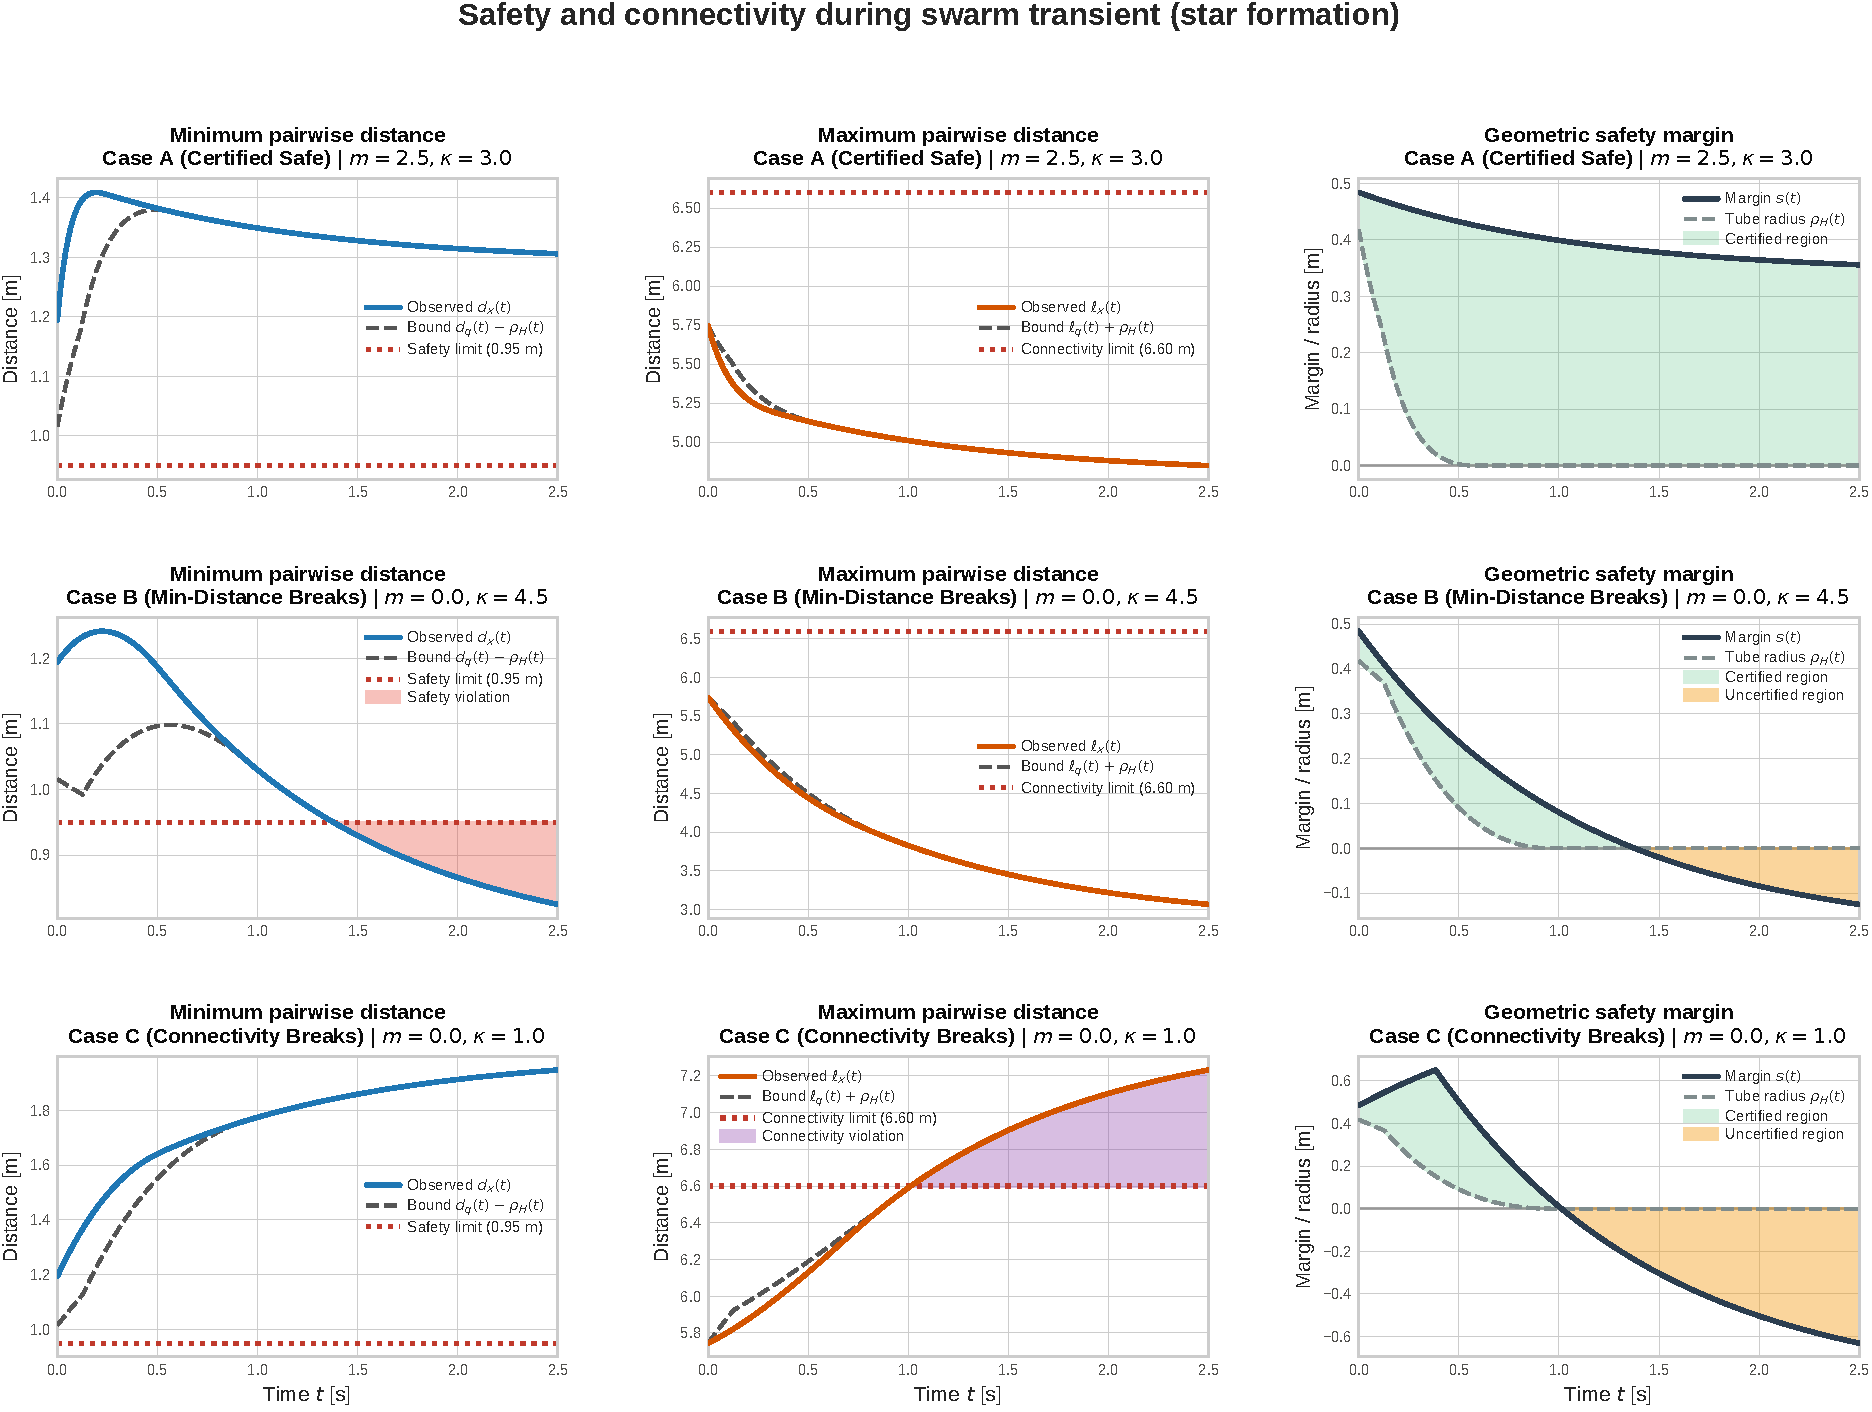
\includegraphics[width=.98\linewidth]{experiment_3/swarm_star_3x3_comparison.pdf}
\caption{Safety and connectivity during swarm transient across the three star-formation cases ($t \in [0, 2.5]$~s). Columns: minimum pairwise distance $d_x(t)$ against $d_q(t)-\rho_H(t)$ and $d_{\rm safe}$ (left), maximum pairwise distance $\ell_x(t)$ against $\ell_q(t)+\rho_H(t)$ and $R_c$ (middle), and geometric safety margin $s(t)$ against distortion radius $\rho_H(t)$ (right).}
\label{fig:star_3x3}
\end{figure}

\section{Coupling--speed parameter map}
Experiment 4 extends the same star template and initial physical state over
the $4\times4$ grid $m\in\{0,1,2,3\}$ and
$\kappa\in\{0.18,1.62,3.06,4.5\}$. Only coupling and compression speed vary;
the reference, thresholds, backbone and 12-unit horizon are shared. For each
point, the analytic condition $1+m w_{\rm lower}\lambda_2(L_H)>\gamma_{\rm req}$
is compared with simulated separation and connectivity. The categories are
$\MapACount$ certified and observed safe/connected (A), $\MapBCount$
uncertified but observed safe/connected (B), and $\MapCCount$ with
observed violations (C), comprising $\MapSeparationCount$ cases with
separation breaches at high compression ($\kappa=4.5$) and
$\MapDisconnectedCount$ cases with connectivity loss at low compression/expansion
($\kappa \in \{0.18, 1.62\}$). There are no certified-case validation failures.
The minimum observed separation is $\MapMinSeparation$; peak full command norms span
$\MapMinPeak$--$\MapMaxPeak$.

The sufficient gain boundary is evaluated over $\kappa \in [0.18, 4.5]$ using
the continuous-time margin calculation: for low $\kappa < 0.95$, rapid formation
expansion renders the margin tube infeasible for certification; across intermediate
speeds $\kappa \in [1.4, 4.0]$, the geometric margins are large enough that uncoupled
tracking ($m=0$) is certified safe; and for $\kappa > 4.1$, rapid compression
requires positive coupling gain, reaching $m \ge 0.4004$ at $\kappa=4.5$. The map
classifies only its 16 simulated points; its colored cells do not certify unsampled
parameter values. All saved adaptive solver nodes were audited, and the closest
observed boundary case retained its classification under tenfold tighter tolerances
and half maximum step.
\begin{figure}[ht]\centering
\IfFileExists{../results/experiment_4/parameter_map.pdf}{\includegraphics[width=.48\linewidth]{experiment_4/parameter_map.pdf}}{\includegraphics[width=.48\linewidth]{parameter_map.pdf}}\hfill
\IfFileExists{../results/experiment_4/parameter_control.pdf}{\includegraphics[width=.48\linewidth]{experiment_4/parameter_control.pdf}}{\includegraphics[width=.48\linewidth]{parameter_control.pdf}}
\caption{Experiment 4 pilot sweep. Left: sampled safety classifications and
continuous-time sufficient gain boundary. Right: peak full physical command.}
\end{figure}

\section{Reproduction and limits}
Run \texttt{python3 run\_experiments.py --experiment 2} to reproduce the coupling gain evaluation.
Run \texttt{python3 run\_experiments.py --experiment 3} from the repository
root to reproduce the star-formation safety and connectivity transient experiment.
Reproduce the parameter map with
\texttt{python3 run\_experiments.py --experiment 4 --grid-size 4 --workers 3}.
The report source is \texttt{ACC\_paper/numerical\_results.tex}; compile it
from \texttt{ACC\_paper/} with \texttt{pdflatex numerical\_results.tex}.
The theoretical source is unchanged. The controller is first order; obstacle
clearance, disturbances, actuator limits and Monte Carlo trials are not
certified or studied here.
\end{document}
